\documentclass{article}\usepackage[]{graphicx}\usepackage[]{color}
%% maxwidth is the original width if it is less than linewidth
%% otherwise use linewidth (to make sure the graphics do not exceed the margin)
\makeatletter
\def\maxwidth{ %
  \ifdim\Gin@nat@width>\linewidth
    \linewidth
  \else
    \Gin@nat@width
  \fi
}
\makeatother

\definecolor{fgcolor}{rgb}{0.345, 0.345, 0.345}
\newcommand{\hlnum}[1]{\textcolor[rgb]{0.686,0.059,0.569}{#1}}%
\newcommand{\hlstr}[1]{\textcolor[rgb]{0.192,0.494,0.8}{#1}}%
\newcommand{\hlcom}[1]{\textcolor[rgb]{0.678,0.584,0.686}{\textit{#1}}}%
\newcommand{\hlopt}[1]{\textcolor[rgb]{0,0,0}{#1}}%
\newcommand{\hlstd}[1]{\textcolor[rgb]{0.345,0.345,0.345}{#1}}%
\newcommand{\hlkwa}[1]{\textcolor[rgb]{0.161,0.373,0.58}{\textbf{#1}}}%
\newcommand{\hlkwb}[1]{\textcolor[rgb]{0.69,0.353,0.396}{#1}}%
\newcommand{\hlkwc}[1]{\textcolor[rgb]{0.333,0.667,0.333}{#1}}%
\newcommand{\hlkwd}[1]{\textcolor[rgb]{0.737,0.353,0.396}{\textbf{#1}}}%
\let\hlipl\hlkwb

\usepackage{framed}
\makeatletter
\newenvironment{kframe}{%
 \def\at@end@of@kframe{}%
 \ifinner\ifhmode%
  \def\at@end@of@kframe{\end{minipage}}%
  \begin{minipage}{\columnwidth}%
 \fi\fi%
 \def\FrameCommand##1{\hskip\@totalleftmargin \hskip-\fboxsep
 \colorbox{shadecolor}{##1}\hskip-\fboxsep
     % There is no \\@totalrightmargin, so:
     \hskip-\linewidth \hskip-\@totalleftmargin \hskip\columnwidth}%
 \MakeFramed {\advance\hsize-\width
   \@totalleftmargin\z@ \linewidth\hsize
   \@setminipage}}%
 {\par\unskip\endMakeFramed%
 \at@end@of@kframe}
\makeatother

\definecolor{shadecolor}{rgb}{.97, .97, .97}
\definecolor{messagecolor}{rgb}{0, 0, 0}
\definecolor{warningcolor}{rgb}{1, 0, 1}
\definecolor{errorcolor}{rgb}{1, 0, 0}
\newenvironment{knitrout}{}{} % an empty environment to be redefined in TeX

\usepackage{alltt}
\title{Problem Set 3}
\author{Cameron Adams}


\usepackage{float, hyperref}
\usepackage[margin = 1in]{geometry}
\usepackage{graphicx}
\usepackage{sectsty}
\usepackage{hyperref}
\IfFileExists{upquote.sty}{\usepackage{upquote}}{}
\begin{document}
%\SweaveOpts{concordance=TRUE}

\maketitle





\section{On Monday, September 25, section will consist of a discussion of good practices in reproducible
research and computing, led by Andrew and Chris. In preparation, please do the following...}

I read: 
\begin{itemize}
    \item Wilson et.al. (http://arxiv.org/pdf/1210.0530v3.pdf)
    \item Millman and Perez (https://github.com/berkeley-stat243/stat243-fall-2014/blob/master/section/millman-perez.pdf)
\end{itemize}

I try to incorporate good coding practices, reproducible research ideals, etc., into my research work. However, the last stage of research-report production-prevents me from fully incorporating these practices. My lab still mostly uses .doc (or Google docs equivalent) file format to produce and submit research drafts. Do you have advice on how to create elegant/efficient work flow to go from .R/python code to latex typesetting/tables to .doc format without cutting and pasting. This is by far the biggest barrier I've seen to fully incorporating the "R/python computation --> completed journal articles" workflow.

I found "Best Practices for Scientific Computing" informative. My code is usually just for me, and is rarely viewed by others. Despite that, I do try to uses wrappers/functions to prevent repeated copy and pasting code. What are recommendations, besides version control for small changes to code. For example, in the first set of analyses I used one set of covariates, and the next week, I want to change those covariates. Is this a scenario where you’ simply recommend version control, another script (analysis1, analysis2)?
 

\section{DRAMATIS PERSONAE: INSTRUCTOR, STUDENTS, GSI} %prob 2

\subsection{Extract the plays into a character vector or a list, with one element for each play. Skip the information at the start of the file, the first piece (the sonnets), and the last piece (Lover's Complaint).} %prob 2a


\begin{knitrout}
\definecolor{shadecolor}{rgb}{0.969, 0.969, 0.969}\color{fgcolor}\begin{kframe}
\begin{alltt}
\hlcom{#download plays in .txt file}
\hlstd{URL}   \hlkwb{<-} \hlstr{"http://www.gutenberg.org/cache/epub/100/pg100.txt"}
\hlstd{download} \hlkwb{<-} \hlkwd{getURL}\hlstd{(URL)}
\hlstd{txt} \hlkwb{<-} \hlstd{download[}\hlnum{1}\hlstd{]}

\hlcom{#############}
\hlcom{#extract plays from "the sonnets" to "lover's complaint"}

\hlcom{#each starts with year published (eg., 1609)}
\hlstd{id} \hlkwb{<-} \hlkwd{str_extract_all}\hlstd{(txt,} \hlstr{"\textbackslash{}\textbackslash{}n[0-9]\{4\}\textbackslash{}\textbackslash{}r"}\hlstd{)[[}\hlnum{1}\hlstd{]]}

\hlcom{#each play also appears to end with "THE END"}
\hlstd{theEnd} \hlkwb{<-} \hlkwd{str_extract_all}\hlstd{(txt,} \hlstr{"THE END"}\hlstd{)[[}\hlnum{1}\hlstd{]]}
\hlkwd{length}\hlstd{(id)}\hlopt{==}\hlkwd{length}\hlstd{(theEnd)} \hlcom{#there are 38 works in this txt file}
\end{alltt}
\begin{verbatim}
## [1] TRUE
\end{verbatim}
\begin{alltt}
\hlcom{##set custom delimter for start of plays}
\hlstd{txt}\hlkwb{<-}\hlkwd{str_replace_all}\hlstd{(txt,} \hlstr{"\textbackslash{}\textbackslash{}n([0-9]\{4\}[\textbackslash{}\textbackslash{}r\textbackslash{}\textbackslash{}n]+)"}\hlstd{,}
                      \hlstr{"\textbackslash{}\textbackslash{}|\textbackslash{}\textbackslash{}|\textbackslash{}\textbackslash{}1"}\hlstd{)}
\hlkwd{length}\hlstd{(}\hlkwd{str_extract_all}\hlstd{(txt,} \hlstr{"\textbackslash{}\textbackslash{}|\textbackslash{}\textbackslash{}|"}\hlstd{)[[}\hlnum{1}\hlstd{]])} \hlcom{#38 delimeters}
\end{alltt}
\begin{verbatim}
## [1] 38
\end{verbatim}
\begin{alltt}
\hlcom{#Set custom delimter for end of plays}
\hlstd{txt}\hlkwb{<-}\hlkwd{str_replace_all}\hlstd{(txt,} \hlstr{"THE END"}\hlstd{,} \hlstr{"THE END\textbackslash{}\textbackslash{}|\textbackslash{}\textbackslash{}|"}\hlstd{)}
\hlkwd{length}\hlstd{(}\hlkwd{str_extract_all}\hlstd{(txt,} \hlstr{"THE END\textbackslash{}\textbackslash{}|\textbackslash{}\textbackslash{}|"}\hlstd{)[[}\hlnum{1}\hlstd{]])} \hlcom{#38 delimeters}
\end{alltt}
\begin{verbatim}
## [1] 38
\end{verbatim}
\begin{alltt}
\hlcom{#fix inconsistenances and remove extraneous repeated text}
\hlstd{txt}\hlkwb{<-}\hlkwd{str_replace_all}\hlstd{(txt,} \hlstr{"ACT [0-9]\{1,2\}\textbackslash{}\textbackslash{}."}\hlstd{,} \hlstr{"ACT I."}\hlstd{)} \hlcom{#ACT 1 -> ACT I.}
\hlstd{txt}\hlkwb{<-}\hlkwd{str_replace_all}\hlstd{(txt,} \hlstr{"Dramatis Personae"}\hlstd{,} \hlstr{"DRAMATIS PERSONAE"}\hlstd{)}
\hlstd{txt} \hlkwb{<-} \hlkwd{str_replace_all}\hlstd{(txt,} \hlstr{"Scene"}\hlstd{,} \hlstr{"SCENE"}\hlstd{)}
\hlstd{txt} \hlkwb{<-} \hlkwd{str_replace_all}\hlstd{(txt,} \hlstr{"Scene:"}\hlstd{,} \hlstr{"SCENE:"}\hlstd{)}
\hlstd{txt}\hlkwb{=}\hlkwd{str_replace_all}\hlstd{(txt,}\hlstr{"<<[\textbackslash{}\textbackslash{}s[:alnum:][:punct:]]*>>"}\hlstd{,}\hlstr{""}\hlstd{)} \hlcom{#remove copyright }

\hlcom{#we've isolated the extranous text with delimeters }
\hlstd{plays} \hlkwb{<-} \hlkwd{unlist}\hlstd{(}\hlkwd{strsplit}\hlstd{(txt,} \hlkwc{split}\hlstd{=}\hlstr{"\textbackslash{}\textbackslash{}|\textbackslash{}\textbackslash{}|"}\hlstd{))} \hlcom{#odd numbered elements can be removed}
\hlstd{plays} \hlkwb{<-} \hlstd{plays[}\hlkwd{seq}\hlstd{(}\hlnum{4}\hlstd{, (}\hlkwd{length}\hlstd{(plays)}\hlopt{-}\hlnum{2}\hlstd{),} \hlnum{2}\hlstd{)]} \hlcom{#remove first/last sonnets}

\hlcom{#now we have all the plays as elements of a character vector}
\hlkwd{substr}\hlstd{(plays[}\hlnum{1}\hlstd{],} \hlnum{0}\hlstd{,} \hlnum{50}\hlstd{)}
\end{alltt}
\begin{verbatim}
## [1] "1603\r\n\r\nALLS WELL THAT ENDS WELL\r\n\r\nby William Sha"
\end{verbatim}
\begin{alltt}
\hlkwd{substr}\hlstd{(plays[}\hlnum{2}\hlstd{],} \hlnum{0}\hlstd{,} \hlnum{50}\hlstd{)}
\end{alltt}
\begin{verbatim}
## [1] "1607\r\n\r\nTHE TRAGEDY OF ANTONY AND CLEOPATRA\r\n\r\nby "
\end{verbatim}
\begin{alltt}
\hlkwd{substr}\hlstd{(plays[}\hlkwd{length}\hlstd{(plays)],} \hlnum{0}\hlstd{,} \hlnum{50}\hlstd{)}
\end{alltt}
\begin{verbatim}
## [1] "1611\r\n\r\nTHE WINTER'S TALE\r\n\r\nby William Shakespear"
\end{verbatim}
\begin{alltt}
\hlcom{#removing the 4th play, "THE COMEDY OF ERRORS" and }
\hlcom{# and "THE SECOND PART OF KING HENRY THE SIXTH" I can't process properly}
\hlstd{plays} \hlkwb{<-} \hlstd{plays[}\hlopt{-}\hlkwd{c}\hlstd{(}\hlnum{4}\hlstd{,}\hlnum{12}\hlstd{)]}
\end{alltt}
\end{kframe}
\end{knitrout}

\subsection{Extract meta data about each play and extract the body of the play. The result should be in the form of an R object, with one element for each play. By meta data I mean the year of the play, the title, the number of acts, and the number of scenes.} %prob2b

\begin{knitrout}
\definecolor{shadecolor}{rgb}{0.969, 0.969, 0.969}\color{fgcolor}\begin{kframe}
\begin{alltt}
\hlcom{############}

\hlcom{#extract metadata}
\hlcom{#titles}
\hlstd{title} \hlkwb{<-} \hlkwd{sapply}\hlstd{(}\hlnum{1}\hlopt{:}\hlkwd{length}\hlstd{(plays),} \hlkwa{function}\hlstd{(}\hlkwc{x}\hlstd{)} \hlkwd{str_extract}\hlstd{(plays[x],} \hlstr{"[^0-9\textbackslash{}\textbackslash{}r\textbackslash{}\textbackslash{}n]+"}\hlstd{))}

\hlcom{#year}
\hlstd{year} \hlkwb{<-} \hlkwd{sapply}\hlstd{(}\hlnum{1}\hlopt{:}\hlkwd{length}\hlstd{(plays),} \hlkwa{function}\hlstd{(}\hlkwc{x}\hlstd{)} \hlkwd{str_extract}\hlstd{(plays[x],} \hlstr{"^[0-9]\{4\}"}\hlstd{))}

\hlcom{#num act per play}
\hlstd{acts} \hlkwb{<-} \hlkwd{sapply}\hlstd{(}\hlnum{1}\hlopt{:}\hlkwd{length}\hlstd{(plays),} \hlkwa{function}\hlstd{(}\hlkwc{x}\hlstd{)}
  \hlkwd{length}\hlstd{(}\hlkwd{unique}\hlstd{(}\hlkwd{c}\hlstd{(}\hlkwd{str_extract_all}\hlstd{(plays[x],} \hlstr{"ACT [IV]\{0,3\}\textbackslash{}\textbackslash{}."}\hlstd{,} \hlkwc{simplify} \hlstd{= T)))))}

\hlcom{#num scenes per play}
\hlstd{scenes} \hlkwb{<-} \hlkwd{sapply}\hlstd{(}\hlnum{1}\hlopt{:}\hlkwd{length}\hlstd{(plays),} \hlkwa{function}\hlstd{(}\hlkwc{x}\hlstd{)}
  \hlkwd{length}\hlstd{(}\hlkwd{c}\hlstd{(}\hlkwd{str_extract_all}\hlstd{(plays[x],} \hlstr{"SCENE\textbackslash{}\textbackslash{}s[0-9IV]\{1,3\}"}\hlstd{,} \hlkwc{simplify} \hlstd{= T))))}
\hlcom{#str_extract_all(plays[3], "SCENE\textbackslash{}\textbackslash{}s[0-9IV]\{1,3\}\textbackslash{}\textbackslash{}.", simplify = T)}

\hlcom{#combine and view}
\hlstd{metaData} \hlkwb{<-} \hlkwd{list}\hlstd{(}\hlkwc{year} \hlstd{= year,} \hlkwc{title} \hlstd{= title,} \hlkwc{acts} \hlstd{= acts,} \hlkwc{scenes} \hlstd{= scenes)}

\hlcom{############}
\hlcom{#extract body of play}
\hlstd{body}\hlkwb{=}\hlkwd{sapply}\hlstd{(}\hlnum{1}\hlopt{:}\hlkwd{length}\hlstd{(plays),} \hlkwa{function}\hlstd{(}\hlkwc{x}\hlstd{)}
  \hlkwd{str_extract_all}\hlstd{(plays[x],}\hlstr{"SCENE(:|\textbackslash{}\textbackslash{}.)([[:alnum:][:punct:]\textbackslash{}\textbackslash{}s]+)"}\hlstd{,}\hlkwc{simplify}\hlstd{=T))}
\end{alltt}
\end{kframe}
\end{knitrout}


\subsection{Extract the actual text spoken by the characters into your object.} %prob 2c


\begin{knitrout}
\definecolor{shadecolor}{rgb}{0.969, 0.969, 0.969}\color{fgcolor}\begin{kframe}
\begin{alltt}
\hlcom{############}
\hlcom{#extract chunks}
\hlstd{extractChunks} \hlkwb{<-} \hlkwa{function}\hlstd{(}\hlkwc{x}\hlstd{) \{}

    \hlcom{#extract speaking chunks}
    \hlstd{chunks} \hlkwb{<-} \hlkwd{str_extract_all}\hlstd{(body[x],} \hlstr{"(?<=\textbackslash{}\textbackslash{}r\textbackslash{}\textbackslash{}n\textbackslash{}\textbackslash{}s\{2\})([^%]+?)(\textbackslash{}\textbackslash{}r\textbackslash{}\textbackslash{}n(?!\textbackslash{}\textbackslash{}s\{4\}))"}\hlstd{,}
                              \hlkwc{simplify} \hlstd{= T)}

    \hlcom{#remove act, scene, stage directions, etc.}
    \hlstd{chunks} \hlkwb{<-} \hlstd{chunks[}\hlopt{-}\hlkwd{grep}\hlstd{(}\hlstr{"(ACT|SCENE|Enter|Exit|ENTER|EXIT)"}\hlstd{, chunks)]}

    \hlkwd{return}\hlstd{(chunks)} \hlcom{#return value}
\hlstd{\}}
\hlstd{chunks} \hlkwb{<-} \hlkwd{sapply}\hlstd{(}\hlnum{1}\hlopt{:}\hlkwd{length}\hlstd{(body),} \hlkwc{FUN} \hlstd{= extractChunks)} \hlcom{#chunks for each play}
\end{alltt}
\end{kframe}
\end{knitrout}
Strategy for extracting chunks was to use lookaheads and lookbehind to look for indents at beginning and end of speaking chunks. They start and end with carriage return, new line, and 2 space indent. Continuing indents are 4 spaces. Then removed ACT, and scene information, along with stage directions.
\begin{knitrout}
\definecolor{shadecolor}{rgb}{0.969, 0.969, 0.969}\color{fgcolor}\begin{kframe}
\begin{alltt}
\hlcom{#extract actors}
\hlstd{extractActors} \hlkwb{<-}  \hlkwa{function}\hlstd{(}\hlkwc{x}\hlstd{) \{}

    \hlcom{#search for JOHN., KING JOHN., Rom. , etc}
    \hlstd{actor_pattern} \hlkwb{<-} \hlkwd{paste0}\hlstd{(}\hlstr{"([A-Z]\{1\}[a-z]+?\textbackslash{}\textbackslash{}.\{1\})|"}\hlstd{,}
                            \hlstr{"([A-Z]\{1\}[a-z]+?\textbackslash{}\textbackslash{}s\{1\}[A-Z]\{1\}[a-z]+?\textbackslash{}\textbackslash{}.\{1\})|"}\hlstd{,}
                            \hlstr{"([A-Z ]\{3,\}?\textbackslash{}\textbackslash{}.\{1\})"}\hlstd{)}
    \hlstd{actors} \hlkwb{<-}
        \hlkwd{unique}\hlstd{(}\hlkwd{str_replace}\hlstd{(}
            \hlkwd{str_extract}\hlstd{(chunks[[x]], actor_pattern),}\hlstr{"^\textbackslash{}\textbackslash{}s+"}\hlstd{,} \hlstr{""}\hlstd{))} \hlcom{#remove whitespace}

    \hlcom{#remove NA's}
    \hlstd{actors} \hlkwb{<-} \hlstd{actors[}\hlopt{!}\hlkwd{is.na}\hlstd{(actors)]}

    \hlcom{#remove unwanted stuff}
    \hlstd{bad_actor_pattern} \hlkwb{<-} \hlkwd{paste0}\hlstd{(}\hlstr{"^(ACT|I\textbackslash{}\textbackslash{}.|II|VI|X|"}\hlstd{,}
                                \hlstr{"EPILOGUE|PROLOGUE|ENTER|Enter|"}\hlstd{,}
                                \hlstr{"EXIT|Exit|[[:punct:]])"}\hlstd{)}
    \hlstd{actors} \hlkwb{<-} \hlstd{actors[}\hlopt{!}\hlkwd{grepl}\hlstd{(bad_actor_pattern, actors)]}
\hlstd{\}}
\hlstd{actors} \hlkwb{<-} \hlkwd{sapply}\hlstd{(}\hlnum{1}\hlopt{:}\hlkwd{length}\hlstd{(chunks),} \hlkwc{FUN} \hlstd{= extractActors)}
\end{alltt}
\end{kframe}
\end{knitrout}


Strategy for extracting actors was to search for single words which end with a period, and the removing obvious non-actor results such as NA, ACT, IV, and things that begin with punctuation.

\subsection{Now use the constructed data object to calculate summary statistics about each play. These should include the following: i. The number of unique speakers. ii. The number of spoken chunks. iii. The number of sentences and words spoken and average number of words per chunk. iv. The number of unique words. When extracting words, make sure you remove punctuation such as commas and periods but not apostrophes.} %prob 2d

\subsubsection{The number of unique speakers.}
\begin{knitrout}
\definecolor{shadecolor}{rgb}{0.969, 0.969, 0.969}\color{fgcolor}\begin{kframe}
\begin{alltt}
\hlcom{#numer of actors per play}
\hlstd{num_actors_play} \hlkwb{<-} \hlkwd{unlist}\hlstd{(}\hlkwd{lapply}\hlstd{(actors,} \hlkwa{function}\hlstd{(}\hlkwc{x}\hlstd{)} \hlkwd{length}\hlstd{(x)))}
\end{alltt}
\end{kframe}
\end{knitrout}
Length of actor vectors per play gives you these quantities.
\subsubsection{The number of spoken chunks.}
\begin{knitrout}
\definecolor{shadecolor}{rgb}{0.969, 0.969, 0.969}\color{fgcolor}\begin{kframe}
\begin{alltt}
\hlcom{#number of spoken chunks per play}
\hlstd{num_spoken_chunks_play} \hlkwb{<-} \hlkwd{unlist}\hlstd{(}\hlkwd{lapply}\hlstd{(chunks,} \hlkwa{function}\hlstd{(}\hlkwc{x}\hlstd{)} \hlkwd{length}\hlstd{(x)))}
\end{alltt}
\end{kframe}
\end{knitrout}
For number of spoken chunks, I counted the number of elements in each vector of chunks for each play.

\subsubsection{The number of sentences and words spoken and average number of words per chunk.}
\begin{knitrout}
\definecolor{shadecolor}{rgb}{0.969, 0.969, 0.969}\color{fgcolor}\begin{kframe}
\begin{alltt}
\hlcom{#number of setences per play}
\hlstd{num_sentences_play} \hlkwb{<-} \hlkwd{sapply}\hlstd{(}\hlnum{1}\hlopt{:}\hlkwd{length}\hlstd{(chunks),}
       \hlkwa{function}\hlstd{(}\hlkwc{x}\hlstd{)} \hlkwd{sum}\hlstd{(}\hlkwd{unlist}\hlstd{(}\hlkwd{lapply}\hlstd{(}
           \hlkwd{str_extract_all}\hlstd{(chunks[x],}\hlstr{"[//.]+"}\hlstd{),} \hlcom{#extract all periods}
            \hlkwa{function}\hlstd{(}\hlkwc{x}\hlstd{)} \hlkwd{length}\hlstd{(x)}\hlopt{-}\hlnum{1} \hlcom{#apply to each list and remove period for speaker}
\hlstd{))))}
\end{alltt}
\end{kframe}
\end{knitrout}
For number of sentences, I used periods to define if a sentence occurred in a chunk, and I subtracted one to account for actor name at the start of a line.

\begin{knitrout}
\definecolor{shadecolor}{rgb}{0.969, 0.969, 0.969}\color{fgcolor}\begin{kframe}
\begin{alltt}
\hlcom{#number of total words spoken per play}
\hlstd{extractWords} \hlkwb{<-} \hlkwa{function}\hlstd{(}\hlkwc{x}\hlstd{) \{} \hlcom{#input vector of chunk for a play}

    \hlstd{tmp} \hlkwb{<-}
        \hlkwd{sapply}\hlstd{(x,} \hlkwa{function}\hlstd{(}\hlkwc{x}\hlstd{)}
            \hlkwd{str_extract_all}\hlstd{(x,} \hlstr{"([A-Z]\{1\}[a-z']+|[a-z']+)"}\hlstd{)[[}\hlnum{1}\hlstd{]])}
            \hlcom{#takes in vector of chunks for play_n,}
            \hlcom{#extracts words with regex, and then counts them}
            \hlcom{#and then sum}

    \hlcom{#unlist and collapse into single character element per play}
    \hlstd{tmp} \hlkwb{<-} \hlkwd{paste0}\hlstd{(}\hlkwd{unlist}\hlstd{(tmp),} \hlkwc{collapse} \hlstd{=} \hlstr{" "}\hlstd{)}

    \hlcom{#remove unneed stuff and combine into character vector}
    \hlstd{tmp} \hlkwb{<-} \hlkwd{str_extract_all}\hlstd{(tmp,} \hlstr{"[A-z']+[^ ']\{1\}"}\hlstd{)}

    \hlcom{#return charcter vector of words for each play}
    \hlkwd{return}\hlstd{(tmp)}
\hlstd{\}}

\hlcom{#get all words in each play}
\hlstd{words_play} \hlkwb{<-} \hlkwd{sapply}\hlstd{(chunks, extractWords)}

\hlcom{#count number of words in each play}
\hlstd{num_words_play} \hlkwb{<-} \hlkwd{sapply}\hlstd{(words_play,} \hlkwa{function}\hlstd{(}\hlkwc{x}\hlstd{)} \hlkwd{length}\hlstd{(x))}
\end{alltt}
\end{kframe}
\end{knitrout}
For total words spoken, I regex'ed for words in each chunk and counted them.
\begin{knitrout}
\definecolor{shadecolor}{rgb}{0.969, 0.969, 0.969}\color{fgcolor}\begin{kframe}
\begin{alltt}
\hlcom{#get num words per chunk per play}
\hlstd{avg_num_words_chunk_play} \hlkwb{<-} \hlstd{num_words_play} \hlopt{/}
                                \hlkwd{sapply}\hlstd{(chunks,} \hlkwa{function}\hlstd{(}\hlkwc{x}\hlstd{)} \hlkwd{length}\hlstd{(x))}
\end{alltt}
\end{kframe}
\end{knitrout}
For average number of words per chunk, simply divide number of words per play by number of chunks per play.


\subsubsection{The number of unique words.}
\begin{knitrout}
\definecolor{shadecolor}{rgb}{0.969, 0.969, 0.969}\color{fgcolor}\begin{kframe}
\begin{alltt}
\hlcom{#num. unique words per play}
\hlstd{num_uniq_words_play} \hlkwb{<-} \hlkwd{sapply}\hlstd{(words_play,} \hlkwa{function}\hlstd{(}\hlkwc{x}\hlstd{)} \hlkwd{length}\hlstd{(}\hlkwd{unique}\hlstd{(x)))}
\end{alltt}
\end{kframe}
\end{knitrout}
For number of unique words, I used the character vector of words from earlier, removed duplicates, and then counted remaining unique words.

\subsection{Plot some of your summary statistics as a function of time...} %prob 2e

\begin{knitrout}
\definecolor{shadecolor}{rgb}{0.969, 0.969, 0.969}\color{fgcolor}\begin{kframe}
\begin{alltt}
\hlcom{#plot fxn}
\hlstd{pplot} \hlkwb{<-} \hlkwa{function}\hlstd{(}\hlkwc{x}\hlstd{,} \hlkwc{y}\hlstd{,} \hlkwc{pch} \hlstd{=} \hlnum{16}\hlstd{,} \hlkwc{cex} \hlstd{=} \hlkwa{NULL}\hlstd{,}
                  \hlkwc{xlab} \hlstd{=} \hlstr{""}\hlstd{,} \hlkwc{ylab} \hlstd{=} \hlstr{""}\hlstd{,} \hlkwc{xaxt} \hlstd{=} \hlstr{"n"}\hlstd{,}
                  \hlkwc{yaxt} \hlstd{=} \hlstr{"n"}\hlstd{,} \hlkwc{bty} \hlstd{=} \hlstr{"n"}\hlstd{,} \hlkwc{...}\hlstd{) \{}

  \hlkwd{plot}\hlstd{(x, y,} \hlkwc{pch} \hlstd{= pch,} \hlkwc{cex} \hlstd{= cex,} \hlkwc{xlab} \hlstd{= xlab,} \hlkwc{ylab} \hlstd{= ylab,}
       \hlkwc{xaxt} \hlstd{= xaxt,} \hlkwc{yaxt} \hlstd{= yaxt,} \hlkwc{bty} \hlstd{=} \hlstr{"n"}\hlstd{,...)}
  \hlkwd{axis}\hlstd{(}\hlnum{1}\hlstd{)}
  \hlkwd{axis}\hlstd{(}\hlnum{2}\hlstd{,} \hlkwc{las} \hlstd{=} \hlnum{2}\hlstd{)}

\hlstd{\}}
\hlkwd{par}\hlstd{(}\hlkwc{mar} \hlstd{=} \hlkwd{c}\hlstd{(}\hlnum{5}\hlstd{,} \hlnum{5}\hlstd{,} \hlnum{4}\hlstd{,} \hlnum{1}\hlstd{),} \hlkwc{mfrow} \hlstd{=} \hlkwd{c}\hlstd{(}\hlnum{3}\hlstd{,} \hlnum{2}\hlstd{))} \hlcom{#set plotting area}
\hlcom{#plot chracteristics of plays}
\hlkwd{pplot}\hlstd{(}\hlkwc{x} \hlstd{= year[}\hlkwd{order}\hlstd{(year)],} \hlkwc{y} \hlstd{= num_actors_play[}\hlkwd{order}\hlstd{(year)],}
      \hlkwc{xlab} \hlstd{=} \hlstr{"Year published"}\hlstd{,} \hlkwc{ylab} \hlstd{=} \hlstr{"Num. actors per play"}\hlstd{,}
      \hlkwc{main} \hlstd{=} \hlstr{"Num. actors per play \textbackslash{}nby time"}\hlstd{)}
\hlkwd{pplot}\hlstd{(}\hlkwc{x} \hlstd{= year[}\hlkwd{order}\hlstd{(year)],} \hlkwc{y} \hlstd{= num_spoken_chunks_play[}\hlkwd{order}\hlstd{(year)],}
      \hlkwc{xlab} \hlstd{=} \hlstr{"Year published"}\hlstd{,} \hlkwc{ylab} \hlstd{=} \hlstr{"Num. spoken chunks per play"}\hlstd{,}
      \hlkwc{main} \hlstd{=} \hlstr{"Num. spoken chunks per play \textbackslash{}nby time"}\hlstd{)}
\hlkwd{pplot}\hlstd{(}\hlkwc{x} \hlstd{= year[}\hlkwd{order}\hlstd{(year)],} \hlkwc{y} \hlstd{= num_sentences_play[}\hlkwd{order}\hlstd{(year)],}
      \hlkwc{xlab} \hlstd{=} \hlstr{"Year published"}\hlstd{,} \hlkwc{ylab} \hlstd{=} \hlstr{"Num. sentences per play"}\hlstd{,}
      \hlkwc{main} \hlstd{=} \hlstr{"Num. sentences per play \textbackslash{}nby time"}\hlstd{)}
\hlkwd{pplot}\hlstd{(}\hlkwc{x} \hlstd{= year[}\hlkwd{order}\hlstd{(year)],} \hlkwc{y} \hlstd{= num_words_play[}\hlkwd{order}\hlstd{(year)]}\hlopt{/}\hlnum{1000}\hlstd{,}
      \hlkwc{xlab} \hlstd{=} \hlstr{"Year published"}\hlstd{,} \hlkwc{ylab} \hlstd{=} \hlstr{"Num. words per play \textbackslash{}n (Thousands)"}\hlstd{,}
      \hlkwc{main} \hlstd{=} \hlstr{"Num. words per play \textbackslash{}nby time"}\hlstd{)}
\hlkwd{pplot}\hlstd{(}\hlkwc{x} \hlstd{= year[}\hlkwd{order}\hlstd{(year)],} \hlkwc{y} \hlstd{= avg_num_words_chunk_play[}\hlkwd{order}\hlstd{(year)],}
      \hlkwc{xlab} \hlstd{=} \hlstr{"Year published"}\hlstd{,} \hlkwc{ylab} \hlstd{=} \hlstr{"Mean num. words per chunk"}\hlstd{,}
      \hlkwc{main} \hlstd{=} \hlstr{"Mean num. words per chunk \textbackslash{}nper play by time"}\hlstd{)}
\hlkwd{pplot}\hlstd{(}\hlkwc{x} \hlstd{= year[}\hlkwd{order}\hlstd{(year)],} \hlkwc{y} \hlstd{= num_uniq_words_play[}\hlkwd{order}\hlstd{(year)],}
      \hlkwc{xlab} \hlstd{=} \hlstr{"Year published"}\hlstd{,} \hlkwc{ylab} \hlstd{=} \hlstr{"Num. unique words per play"}\hlstd{,}
      \hlkwc{main} \hlstd{=} \hlstr{"Num. unique words \textbackslash{}nper play by time"}\hlstd{)}
\end{alltt}
\end{kframe}
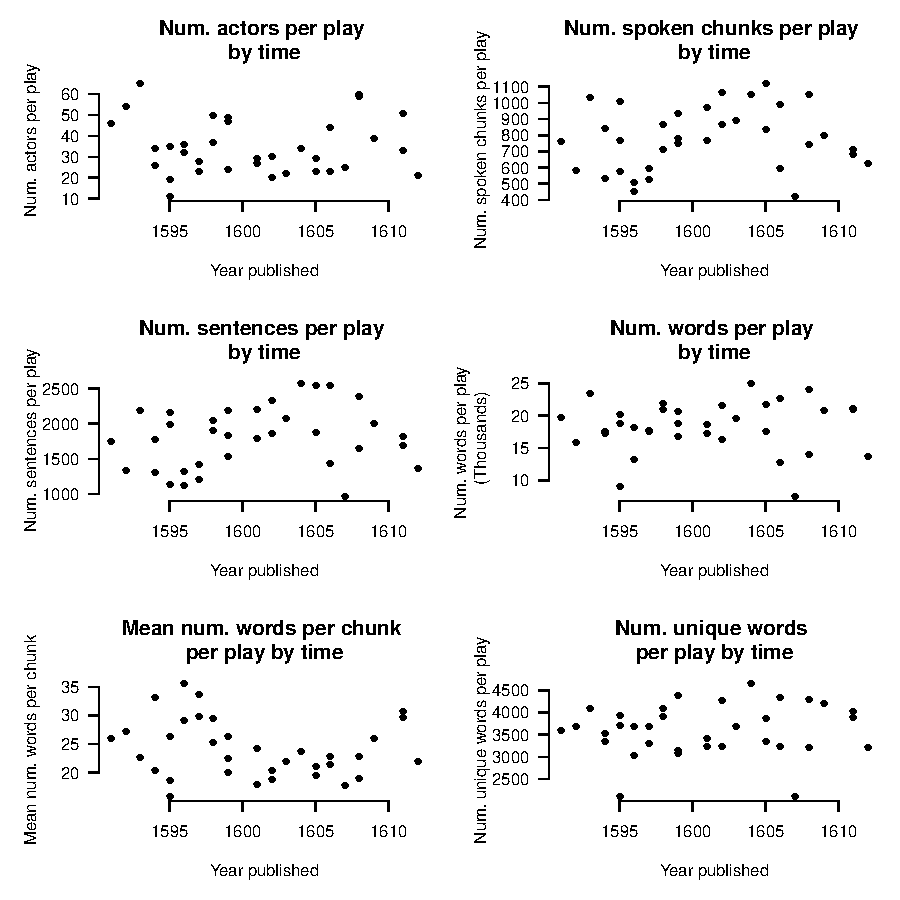
\includegraphics[width=\maxwidth]{figure/unnamed-chunk-12-1} 
\begin{kframe}\begin{alltt}
\hlkwd{par}\hlstd{(}\hlkwc{mar} \hlstd{=} \hlkwd{c}\hlstd{(}\hlnum{5}\hlstd{,} \hlnum{4}\hlstd{,} \hlnum{4}\hlstd{,} \hlnum{1}\hlstd{),} \hlkwc{mfrow} \hlstd{=} \hlkwd{c}\hlstd{(}\hlnum{1}\hlstd{,}\hlnum{1}\hlstd{))}
\end{alltt}
\end{kframe}
\end{knitrout}

Plots don't indicate any obvious time trends, but the number of spoken chunks, and number of sentences peaked around year 1605, at the same time the number of words per chunk was at its smallest. The number of actors, unique words, and number of words were generally consistently noisy.


\begin{kframe}
\begin{alltt}
\hlcom{#combine num. of acts and scenes, unique speakers, chunks for each play}
\hlstd{report} \hlkwb{<-} \hlkwd{cbind}\hlstd{(acts, scenes, num_actors_play, num_spoken_chunks_play)[}\hlkwd{order}\hlstd{(year),]}

\hlkwd{colnames}\hlstd{(report)} \hlkwb{<-} \hlkwd{c}\hlstd{(}\hlstr{"Acts"}\hlstd{,} \hlstr{"Scenes"}\hlstd{,} \hlstr{"Actors"}\hlstd{,} \hlstr{"Spoken chunks"}\hlstd{)}
\hlkwd{rownames}\hlstd{(report)} \hlkwb{<-} \hlkwd{substr}\hlstd{(title[}\hlkwd{order}\hlstd{(year)],} \hlnum{0}\hlstd{,} \hlnum{20}\hlstd{)} \hlcom{#shorten titles to fit}

\hlcom{#print table of characteristics}
\hlkwd{require}\hlstd{(xtable)}
\hlstd{tbl} \hlkwb{<-} \hlkwd{xtable}\hlstd{(report,} \hlkwc{caption} \hlstd{=} \hlstr{"Characteristics of Shapkespeare plays extracted using regex"}\hlstd{,}
           \hlkwc{comment} \hlstd{= F,} \hlkwc{align} \hlstd{=} \hlkwd{c}\hlstd{(}\hlstr{"l"}\hlstd{,} \hlkwd{rep}\hlstd{(}\hlstr{"c"}\hlstd{,} \hlkwd{dim}\hlstd{(report)[}\hlnum{2}\hlstd{])))}
\hlkwd{print}\hlstd{(tbl,} \hlkwc{floating} \hlstd{= T,} \hlkwc{table.placement} \hlstd{=} \hlstr{"H"}\hlstd{,} \hlkwc{comment} \hlstd{= F,}
      \hlkwc{row.names} \hlstd{= T,} \hlkwc{caption.placement} \hlstd{=} \hlstr{"top"}\hlstd{,} \hlkwc{caption.width} \hlstd{=} \hlstr{"35em"}\hlstd{)}
\end{alltt}
\end{kframe}\begin{table}[H]
\centering
\parbox{35em}{\caption{Characteristics of Shapkespeare plays extracted using regex}} 
\begin{tabular}{lcccc}
  \hline
 & Acts & Scenes & Actors & Spoken chunks \\ 
  \hline
THE THIRD PART OF KI &   5 &  28 &  46 & 760 \\ 
  THE FIRST PART OF HE &   5 &  27 &  54 & 585 \\ 
  KING RICHARD III &   5 &  25 &  65 & 1034 \\ 
  THE TAMING OF THE SH &   4 &  14 &  34 & 841 \\ 
  THE TRAGEDY OF TITUS &   5 &  14 &  26 & 532 \\ 
  LOVE'S LABOUR'S LOST &   5 &   9 &  19 & 1012 \\ 
  THE TRAGEDY OF ROMEO &   5 &  24 &  35 & 768 \\ 
  THE TWO GENTLEMEN OF &   5 &  20 &  11 & 575 \\ 
  A MIDSUMMER NIGHT'S  &   5 &   9 &  32 & 454 \\ 
  KING RICHARD THE SEC &   5 &  19 &  36 & 510 \\ 
  KING JOHN &   5 &  16 &  28 & 525 \\ 
  THE MERCHANT OF VENI &   5 &  20 &  23 & 592 \\ 
  THE FIRST PART OF KI &   5 &  19 &  37 & 712 \\ 
  SECOND PART OF KING  &   5 &  19 &  50 & 866 \\ 
  THE LIFE OF KING HEN &   5 &  23 &  47 & 783 \\ 
  THE TRAGEDY OF JULIU &   5 &  18 &  49 & 749 \\ 
  MUCH ADO ABOUT NOTHI &   5 &  17 &  24 & 938 \\ 
  AS YOU LIKE IT &   5 &  22 &  27 & 770 \\ 
  THE MERRY WIVES OF W &   4 &  23 &  29 & 970 \\ 
  THE HISTORY OF TROIL &   5 &  24 &  30 & 1063 \\ 
  TWELFTH NIGHT; OR, W &   5 &  18 &  20 & 868 \\ 
  ALLS WELL THAT ENDS  &   5 &  23 &  22 & 890 \\ 
  THE TRAGEDY OF HAMLE &   4 &  20 &  34 & 1052 \\ 
  MEASURE FOR MEASURE &   4 &  17 &  23 & 839 \\ 
  THE TRAGEDY OF OTHEL &   5 &  15 &  29 & 1119 \\ 
  THE TRAGEDY OF KING  &   5 &  26 &  23 & 991 \\ 
  THE TRAGEDY OF MACBE &   5 &  29 &  44 & 593 \\ 
  THE TRAGEDY OF ANTON &   5 &  32 &  25 & 421 \\ 
  THE TRAGEDY OF CORIO &   5 &  28 &  60 & 1055 \\ 
  THE LIFE OF TIMON OF &   5 &  17 &  59 & 743 \\ 
  CYMBELINE &   5 &  27 &  39 & 801 \\ 
  KING HENRY THE EIGHT &   5 &  17 &  51 & 684 \\ 
  THE WINTER'S TALE &   5 &  15 &  33 & 713 \\ 
  THE TEMPEST &   5 &   9 &  21 & 623 \\ 
   \hline
\end{tabular}
\end{table}


\subsection{Extra credit:} %prob 2f

\section{This problem asks you to design an object-oriented programming (OOP) approach to the Shakespeare analysis of problem 2.}

\subsection{What are the fields (i.e., member data, slots, etc.) for the class? ...} %prof 3a

The fields would be the objects containing parts of each play (or one with the entire plays) and objects with metadata about the plays (title, number of acts, year published, etc.). Going with the suggestion in the question, there could also be an array object which is comprised of the components of each play. And we use these components of each play to extract information about the play, such as number of chunks, actors, etc.

Example of  object structure:
\begin{itemize}
    \item plays (array which contains lists of components of each play)
    \begin{itemize}
        \item body (list of character vectors, each element the body only of a play)
        \item chunks (list of character vectors)
        \item actors (list of character vectors)
        \item titles (list of character vectors)
    \end{itemize}
\end{itemize}   

We would then need a field for the meta Data (list) we wish to extract from the plays array
\begin{itemize}
    \item meta Data (list of integer vectors)
    \begin{itemize}
        \item num\_actors (integer vector)
        \item num\_acts (integer vector)
        \item num\_scenes (integer vector)
        \item num\_words (integer vector)
        \item num\_sentences (integer vector)
        \item ..., etc.
    \end{itemize}
\end{itemize}


\subsection{What are the methods for the class? ...} %prof 3b

First we would have methods which would process the plays into its components (titles, body, actors, chunks, etc.)

Example pseudo code:

\begin{knitrout}
\definecolor{shadecolor}{rgb}{0.969, 0.969, 0.969}\color{fgcolor}\begin{kframe}
\begin{alltt}
\hlcom{#Input: Entire text downloaded from web}
\hlcom{#Output: list of plays}
\hlstd{processWebData} \hlkwb{<-} \hlkwa{function}\hlstd{(}\hlkwc{EntireText}\hlstd{) \{}

    \hlstd{plays} \hlkwb{<-} \hlkwd{getPlays}\hlstd{(EntireText)}           \hlcom{#subset plays}

    \hlkwd{return}\hlstd{(plays)}                           \hlcom{#return a list of plays)   }
\hlstd{\}}

\hlcom{#Input: list of plays}
\hlcom{#Output: array of plays with their component parts}
\hlstd{processWebData} \hlkwb{<-} \hlkwa{function}\hlstd{(}\hlkwc{plays}\hlstd{) \{}

    \hlstd{titles} \hlkwb{<-} \hlkwd{getTitles}\hlstd{(plays)}              \hlcom{#get titles}

    \hlstd{body} \hlkwb{<-} \hlkwd{getBody}\hlstd{(plays)}                  \hlcom{#get body of plays}

    \hlstd{chunks} \hlkwb{<-} \hlkwd{getChunks}\hlstd{(body)}               \hlcom{#get chunks}

    \hlstd{actors} \hlkwb{<-} \hlkwd{getActors}\hlstd{(chunks)}             \hlcom{#get actors/speakers}

    \hlkwd{return}\hlstd{(}\hlkwd{list}\hlstd{(body, actors,}               \hlcom{#return lists of play components}
                \hlstd{chunks, titles))}

\hlstd{\}}
\end{alltt}
\end{kframe}
\end{knitrout}
Then we would need a method for extracting metaData info from the play components
\begin{knitrout}
\definecolor{shadecolor}{rgb}{0.969, 0.969, 0.969}\color{fgcolor}\begin{kframe}
\begin{alltt}
\hlcom{#intput: plays array}
\hlcom{#output: list of metaData for each play}
\hlstd{extractMetaData} \hlkwb{<-} \hlkwa{function}\hlstd{(}\hlkwc{plays}\hlstd{) \{}

    \hlstd{num_actors} \hlkwb{<-} \hlkwd{extractNumActors}\hlstd{(actors)}

    \hlstd{num_setences} \hlkwb{<-} \hlkwd{extractNumSentences}\hlstd{(body)}

    \hlstd{num_words} \hlkwb{<-} \hlkwd{extractNumWords}\hlstd{(body)}

    \hlstd{...}

    \hlkwd{return}\hlstd{(}\hlkwd{list}\hlstd{(num_actors, num_sentences, num_words, ..., etc.))}
\hlstd{\}}
\end{alltt}
\end{kframe}
\end{knitrout}







\end{document}
